The proposal consist on a possibilistic valid-time model. The representation and the querying are explained in the following subsections.

\subsection{Representation of Ill-known Valid-time Intervals}
\label{subsec:representation-ill-known}
Valid time is usually represented as an interval. The interval has a starting and an ending points. An ill-known valid-time interval is an interval in witch one or both points are ill-known. 

\begin{definition}
A Possibilistic Valid-Time Period \textbf{PVP} is a possibilistic interval defined by means of two ill-known points, namely $\left[ X,\ Y \right]$
\begin{equation}
PVP = \left[X,\ Y \right] 
\end{equation}
$X$ and $Y$ are ill-known values in the set of the real numbers $\mathbb{R}$. The uncertainty about the values taken by $X$ and $Y$ are given by the possibility distributions $\pi_X$ and $\pi_Y$.
\end{definition}

The possibility distributions $\pi_X$ and $\pi_Y$ are given in the way of a triangular distribution, as explained in subsection \ref{subsec:fuzzy-numbers}. This representation allows overlapping (Fig. \ref{fig:pvp}).


\begin{figure}[h!]
  \centering
%  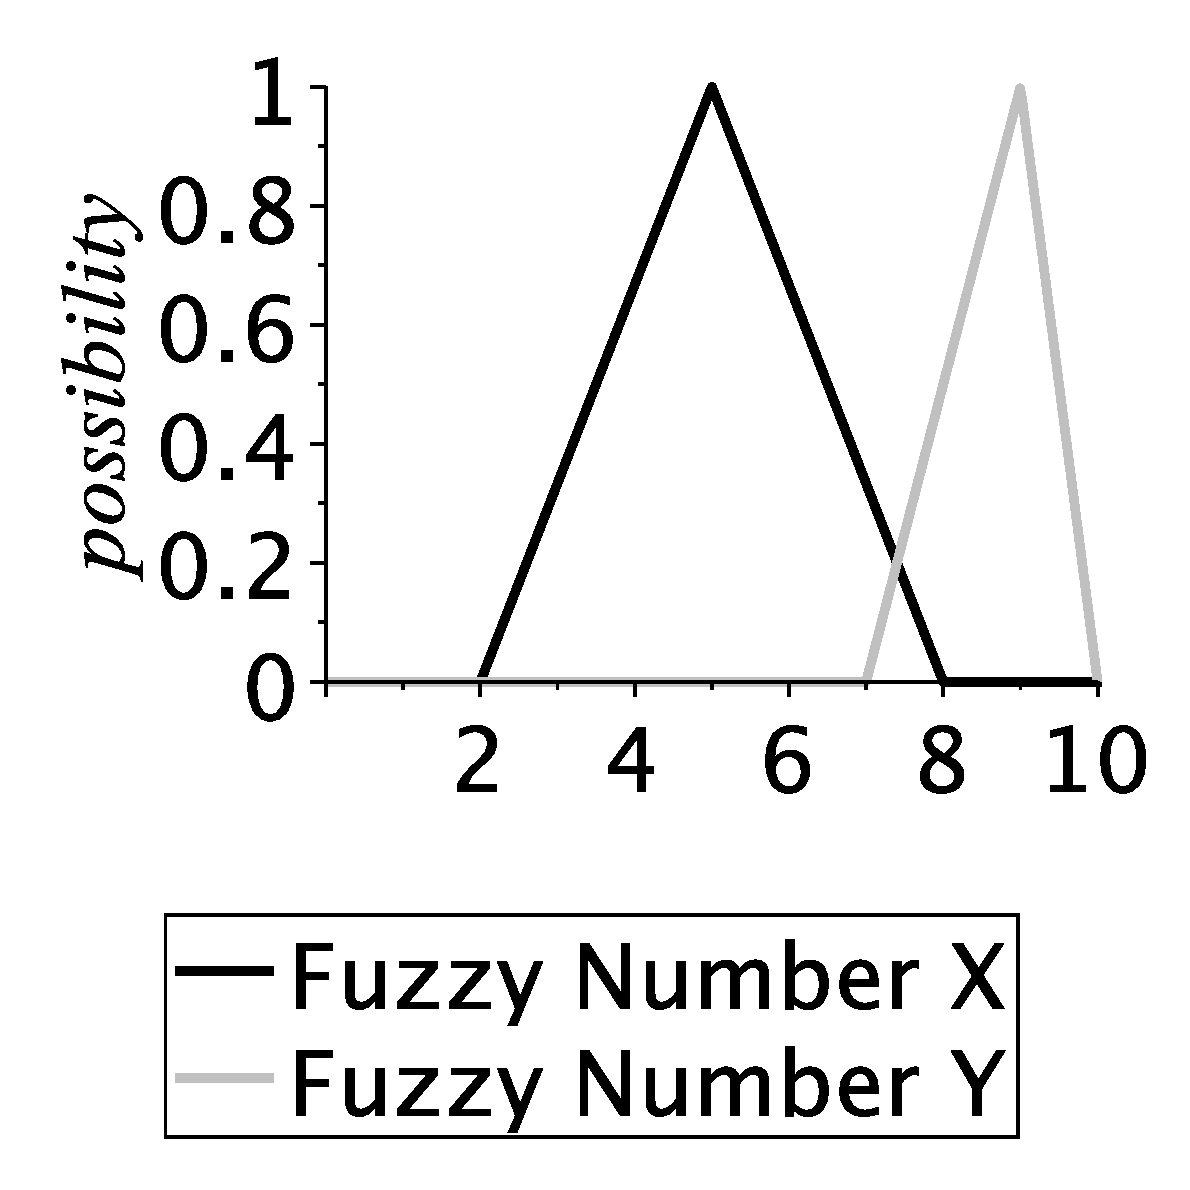
\includegraphics[scale=0.2]{graphs/2_triangular.eps}
  \caption{Two fuzzy numbers $X$ and $Y$ denoting a Possibilistic Valid-Time Period \emph{PVT}.}
  \label{fig:pvp}
\end{figure}

\subsection{Storage of Valid-time Intervals}
\label{subsec:storage}
Each database row containing a \emph{PVP} stores it as two triangular possibility distributions. In our approach we propose the representation of that as proposed in the  fuzzy interface for relational databases \emph{FIRST}~\cite{Medina94gefred.a,Gal98}. In this representation it is also possible to represent not only fuzzy numbers but fuzzy constants (see table \ref{table:relational-representation-pvp}):

\begin{itemize}
\item
\emph{NULL}: This constant refers to a completely ignorance about the value. The possibility distribution for a given fuzzy number $X$ is not defined, therefore, any comparison between a fuzzy number and the \emph{NULL} constant always returns $0$.
\item
\emph{UNKNOWN}: The point has a value but it is unknown. The possibility distribution for a given fuzzy number $X$ is $\pi_X=1$
\item
\emph{UNDEFINED}: The point does not have a value. The possibility distribution for a given fuzzy number $X$ is $\pi_X=0$
\end{itemize}


\begin{table}
\caption{Relational representation for a Possibilistic Valid-Time Period.}
\centering
\begin{tabular}{c c c c c c}
\hline
Value & FT & F1 & F2 & F3  \\ \hline
UNKNOWN & 0 & NULL & NULL & NULL  \\ 
UNDEFINED & 1 & NULL & NULL & NULL  \\ 
NULL & 2 & NULL & NULL & NULL  \\ 
$\left[D,\ a,\ b \right]$ & 3 & $D$ & $D-a$ & $D+b$ \\ 
\hline
\end{tabular}
\label{table:relational-representation-pvp}
\end{table}

\subsection{Querying Ill-known Valid-time Intervals}
In order to provide a complete model, we will provide the tools for querying. This allows the user to specify both the preferences and an ill-known valid-time interval in the query. It is important to notice that the possibilistic / fuzzy data stored in the database has a \emph{disjunctive interpretation} (it is said that we have \emph{uncertainty}: the valid-time interval has only one value but, for some reason the value is ill-known). In the query specification, the user is allowed to express a crisp time interval. In this approach, the interpretation is the following: the user w
In this subsection we will define the query specification, then the evaluation of the query and finally the ranking for the query.

\subsubsection{Query specification}
A query in our framework has two different parts: the first one is the query specification for regular attributes. The second part is the temporal specification. 

\begin{definition}
A query $\tilde Q$ is specified by:
\begin{equation}
\label{eq:query-definition}
\tilde Q = \left( Q^{time}, Q \right)
\end{equation}
\end{definition}
Where $Q$ are the (possibly fuzzy) preferences of the user  and $Q^{time}$ is the temporal part specified by a crisp interval. The temporal part is composed by two arguments:

\begin{definition}
 $Q^{time}$ is composed by:
\begin{equation}
Q^{time} = \left( \left[a, \ b \right] , Ar \right), a,b \in \mathbb{R}
\end{equation}
Where $ \left[a, \ b \right] $ is the specification for the crisp interval and $Ar$ is one of the Allen's relations (table \ref{tab:allen-relations}).
\end{definition}

\begin{table}[h]
\centering
\begin{tabular}{|c|c|c|}
\hline
Allen Relation & Constraints & $\bool(p_1,...,p_n)$ \\
\hline
I before J & $C_1\stackrel{\triangle}{=} \left(<,X\right)$ & $p_1$ \\
\hline
\multirow{4}{*}
{I equal J} & $C_1\stackrel{\triangle}{=} \left(\geq,X\right)$ & \text{$p_1\wedge\neg p_2\wedge p_3\wedge\neg p_4$}\\
 & $C_2\stackrel{\triangle}{=} \left(\neq,X\right)$ & \\
 & $C_3\stackrel{\triangle}{=} \left(\leq,Y\right)$ & \\
 & $C_4\stackrel{\triangle}{=} \left(\neq,Y\right)$ & \\
\hline
\multirow{2}{*}
{I meets J} & $C_1\stackrel{\triangle}{=} \left(\leq,X\right)$ & $p_1\wedge\neg p_2$\\
 & $C_2\stackrel{\triangle}{=} \left(\neq,X\right)$ & \\
\hline
\multirow{3}{*}
{I overlaps J} & $C_1\stackrel{\triangle}{=} \left(<,Y\right)$ & $p_1\wedge\neg p_2\wedge\neg p_3$\\
 & $C_2\stackrel{\triangle}{=} \left(\leq,X\right)$ & \\
 & $C_3\stackrel{\triangle}{=} \left(\geq,X\right)$ & \\
\hline
\multirow{4}{*}
{I during J} & $C_1\stackrel{\triangle}{=} \left(>,X\right)$ & $(p_1\wedge p_2)\vee(p_3\wedge p_4)$\\
 & $C_2\stackrel{\triangle}{=} \left(\leq,Y\right)$ & \\
 & $C_3\stackrel{\triangle}{=} \left(\geq,X\right)$ & \\
 & $C_4\stackrel{\triangle}{=} \left(<,Y\right)$ & \\
\hline
\multirow{2}{*}
{I starts J} & $C_1\stackrel{\triangle}{=} \left(\geq,X\right)$ & $p_1\wedge\neg p_2$\\
 &  $C_2\stackrel{\triangle}{=} \left(\neq,X\right)$ & \\
\hline
\multirow{2}{*}
{I finishes J} & $C_1\stackrel{\triangle}{=} \left(\leq,Y\right)$ & $p_1\wedge\neg p_2$\\
 & $C_2\stackrel{\triangle}{=} \left(\neq,Y\right)$ & \\
\hline
\end{tabular}
\label{tab:allen-relations}
\caption{Allen's relations represented in the framework.}
\end{table}




\subsubsection{Query evaluation}
Fuzzy querying of regular (relational) databases, query satisfaction modelling is a matter of degree. Usually, criteria satisfaction is modelled by means of a satisfaction degree $s \in \left[ 0, 1\right]$. In the model, every record $r$ contains a \emph{PVP} $V_r$ to model the valid-time for that record.

The query evaluation method is the following:
\begin{itemize}
\item
For each record $r$ in the database, the preferences expressed in $Q$ are evaluated in the unit interval. Thus, $e(Q) \in \left[0, 1\right]$ is the evaluation function for the criteria in $Q$.
\item
For each record $r$ in the database, the interval $ \left[a, \ b \right]$ is compared to the $PVP$ value by means of the corresponding Allen relation specified by $ar$. The result is again in the unit interval. Here, $e(Q^{time}) \in \left[0, 1 \right]$ is the evaluation function for the criteria $Q^{time}$.
\end{itemize}


\subsubsection{Ranking}
In order to present the results to the user, a ranking method must be used. Both $Q$ and $Q^{time}$ are evaluated independently and also both are evaluated in the unit interval. The ranking is computed using a convex combination of both values:

\begin{equation}
e(\tilde{Q})\ =\ \omega*e(Q)\ +\ (1-\omega)*e(Q^{time})
\end{equation}
Where $\omega \in \left[0, 1 \right]$. By increasing the value for the parameter $\omega$, the preferences expressed in the query $Q$ can be given more importance. By lowering the value for $\omega$, the temporal criteria is emphasized.
The following example illustrates the querying process.


\begin{example} 

\textbf{The database}
%%%%%%%%%%%%%%%%%%%%%%%%%%%%%%%%%%%%%%%%%%%%%%%%%%
% Sample table for the car models. 
%%%%%%%%%%%%%%%%%%%%%%%%%%%%%%%%%%%%%%%%%%%%%%%%%%%
\begin{table}[ht]
\caption{Sample database containing the car models.}
\centering
\begin{tabular}{c c c c c c c}
\hline
ID & IID & Segment & Manufac. & Name & Start & End  \\ [0.5ex]
\hline
001 & 1 & B & Peugeot & 205 & [1985,2,3] & [1997,2,1] \\
002 & 1 & C & Peugeot & 305 & [1977,2,2] & [1989,2,3] \\
003 & 1 & B & Citroen & C2 & [2003,3,2] & [2006,1,1] \\
001 & 2 & B & Peugeot & 206 & [1998,1,1] & [2011,2,1] \\
001 & 3 & B & Peugeot & 207 & [2006,1,1] & [2011,1,1]\\
\hline
\end{tabular}
\label{tb:car-models}
\end{table}


Consider a database containing car models. There are several general attributes (car model's name, car manufacturer, car segment) and one temporal attribute (which is ill-known) containing the approximate date while the car model was sold. The temporal data is stored as explained in subsection \ref{subsec:storage}. The value for $D$ is stored in \emph{yyyy} format and $a$ and $b$ are represented by an integer, for the convenience of the representation. Therefore the chronons in our example will be years. The ID field identifies a car model while the field Instance ID (IID) identifies the instance for a car model. \\

\textbf{The query}
Consider the following query:

\emph{The user wants to obtain a list of models in the segment B for the manufacturer Peugeot before the year interval 2001-2005.}

The query is translated to the following expression, using the structure given in equation \eqref{eq:query-definition}:

\begin{center}
$\tilde{Q} = \left(  c^{time}, c_{segment} \right)$
\end{center}

Where:
\begin{itemize}
\item
$c^{time}\ = \ ( \left[ 2001,\ 2005 \right],\ $  before $)$.
\item
$c_{segment}\ = \ $ Peugeot.
\end{itemize}

The evaluation for the criteria are presented in the result table \ref{tb:results}.

\begin{table}[ht]
\caption{Result table and ranking}
\centering
\begin{tabular}{c c c c c }
\hline
ID & IID &  $c^{time}$ & $c_{segment}$ & rank ($\omega=0.5$) \\ [0.5ex]
\hline
001 & 1  & 1 & 1 & 1 \\
002 & 1  & 1 & 0 & 0.5 \\
003 & 1  & 0.333  & 0 & 0.166\\
001 & 2 & 1 & 1 & 1 \\
001 & 3 & 0 & 1 & 0.5\\
\hline
\end{tabular}
\label{tb:results}
\end{table}
\end{example}




